\section{The remaining systems boundary}\label{sec:C34:07}
The October 2026 ecosystem makes persistence, tools, skills, and orchestration accessible through increasingly explicit protocol and runtime interfaces. The unresolved boundary is the evidence needed when these mechanisms are composed and updated. MCP conformance describes protocol behavior; it does not certify source truth or permission. Durable execution interfaces describe state management; they do not make every external effect reversible. Serving optimizations improve a resource envelope; they do not guarantee preserved task behavior after context or precision changes. The same distinction applies to scientific agents: an autonomous software loop does not establish autonomous physical experimentation, and a changed assay result does not isolate a changed reasoning policy.

Domain transfer also changes the admissible experiment. Cybersecurity capability in a controlled target environment does not grant authority over another system. Evidence from a noninfectious molecular-discovery sandbox does not establish clinical efficacy or the conditions for a different biological workflow. These boundaries belong to the task definition and evidence record; a larger model, longer session, or successful API call cannot discharge them.

The final research standard is therefore an auditable chain from problem formulation to delivered artifact: define the information available to each decision, identify mutable state and authority, derive the mechanism under explicit assumptions, connect it to an implementation, compare against controlled alternatives, and preserve failures and uncertainty. Where evidence is missing, the conclusion narrows. Where a simple baseline survives, complexity needs a measured justification. Where a current method improves only one layer, its cross-layer consequences remain part of the claim.

Generality will be better understood through experiments that discriminate these mechanisms than through broader labels. The technically productive questions are specific: which distinctions must a memory preserve, which histories a policy was trained on, which cache state remains valid, which operation committed, which verifier requirement was actually tested, and which improvement survives an independent task stream. Answering those questions is the path from a collection of model capabilities to reliable, adaptable agentic systems.


Figure~\ref{fig:C34:overview} isolates the mechanism and its stated information boundaries.
\begin{figure}[!htbp]
\centering
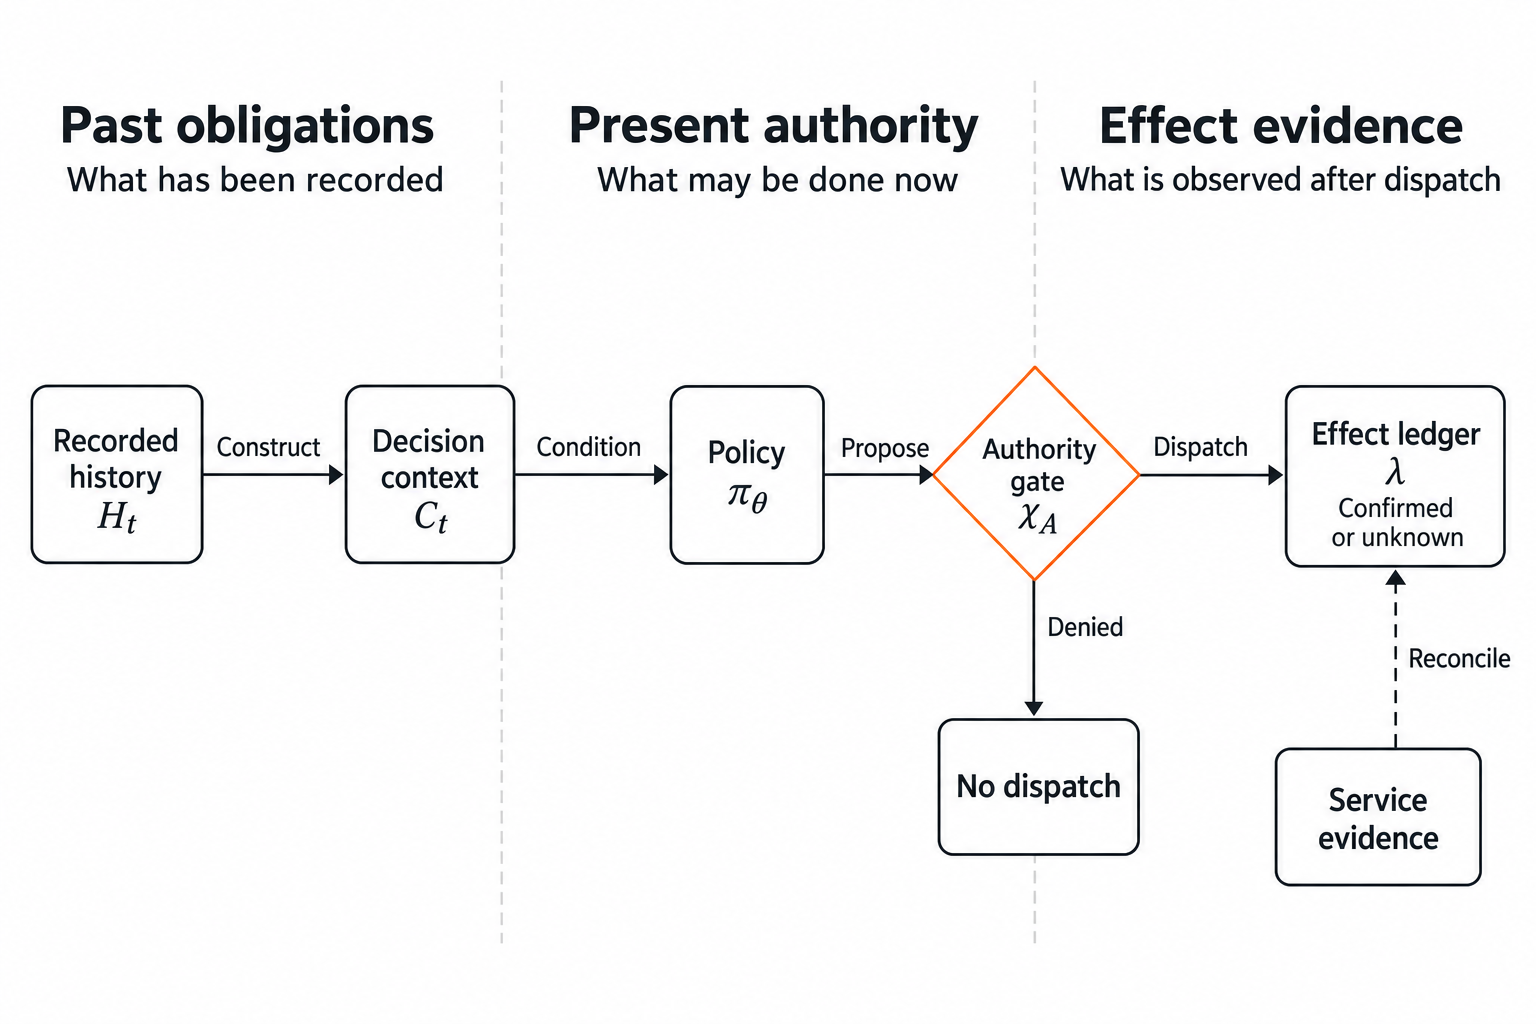
\includegraphics[width=\linewidth]{book/figures/assets/F34review.png}
\caption{State continuity separates the information used by a policy, current dispatch authority and evidence of external effects. Permission does not establish source truth, and an authorized dispatch can leave the effect ledger unknown. Compatibility and independent evaluation are obligations for updates, rather than guarantees inherited from one component score.}
\label{fig:C34:overview}
\end{figure}
